%!TEX root = ../DevaramaniS-[RnD-MT]Report.tex

\chapter{State of the Art}
%\section{....}
%Use as many sections as you need in your related work to group content into logical groups
%
%correctly cite your sources \cite{art1}.

The current state of the art focuses on various approaches to implement complex robot tasks involving robust motions and complex motion primitives. As mentioned earlier (section~\ref{chap:Intro}), the task requirements impose explicit constraints on robot motions. These constraints indicate the desired force or motion to be executed by the robot. It is imperative to consider the dynamic properties of the system to realize these constraints instantaneously and execute the optimal motions. In this section, current state of the art relating to robot dynamic algorithms, task specification formalisms and dynamic solvers are summarized briefly.

\section{Robot dynamics algorithms}
Robot dynamics deals with the relationship between applied force and produced accelerations in the system~\cite{featherstone2014rigid}. The robot dynamics algorithms refer to numerical computations of quantities associated with dynamics. It is well known that the robot dynamics problem is of two types -  forward and inverse dynamics. The forces applied on any rigid body produces acceleration in the direction of applied force, this is termed as \textit{forward dynamics}. The equation used to solve forward dynamics problem is given by~\cite{featherstone2014rigid},
\begin{equation}\label{eq:fd}
	FD \rightarrow M(q)^{-1} (\tau - C(q, \dot{q})) = \ddot{q}
\end{equation}

where, $M(q)$ stands for inertia matrix represented in joint space and is a function of joint position ($q$). $\tau$ denotes the applied force and $C$ is the Centrifugal and Coriolis forces acting on the system. 
 The \textit{inverse dynamics} deals with computation of forces required to produce the desired acceleration. The equation used to solve inverse dynamics problem can be formulated as~\cite{vukcevic2018extending}~\cite{featherstone2014rigid},

\begin{equation}
	\label{eq:ID}
	ID \rightarrow M(q)\ddot{q} + C(q, \ddot{q}) = \tau
\end{equation}

The above equation is also termed as \textit{dynamic equation of motion} for rigid body system (further explanation can be found in appendix~\ref{chap:dynamic}). There are several types of robots such as manipulators, mobile robots, aerial robots etc, which are composition of rigid bodies. In this project, to simplify the analysis of robot dynamics, \textit{Spatial notations} are used to represent the system and follows the convention as used in Featherstone~\cite{featherstone2014rigid}. The Spatial notions include 6D vectors describing six degrees of freedom of a single rigid body. 

The applications of forward dynamics can be found mainly in simulation, whereas, inverse dynamics is applied for motion control system~\cite{featherstone1984robot}. However, there are different robot task definitions that requires combination of forward and inverse dynamics. Specifically for applications involving \textit{posture control} (humanoid robots and manipulators), the robot must realize the motion and force constraints instantaneously as imposed by the task requirements. The basic algorithms to solve each of the dynamics problem are listed below,
\begin{enumerate}
	\item \textit{Forward dynamics}
	\begin{itemize}
		\item \textit{Composite Rigid Body Algorithm (\hyperref[crba]{CRBA})}~\cite{walker1982efficient}: For the given link length, $n < 9$, this method is an efficient algorithm than \hyperref[aba]{ABA}, to compute forward dynamics~\cite{featherstone2000robot}. 
		\item  \textit{Articulated-Body Algorithm (\hyperref[aba]{ABA})}: The method considers whole system as articulated body and computes the forward dynamics. It has \textit{O(n)} computational complexity.
	\end{itemize}
	\item \textit{Inverse dynamics}
	\begin{itemize}
		\item \textit{Recursive Newton-Euler Algorithm (\hyperref[rnea]{RNEA})}: The algorithm is applied to calculate inverse dynamics of a general kinematic tree~\cite{featherstone2000robot}. It involves two passes - \textit{outward} and \textit{inward}. In outward pass, \textit{velocity} and \textit{acceleration} quantities are computed from base to the leaves and \textit{joint forces} are computed from leaves to the root during inward pass~\cite{featherstone2014rigid}. 
	\end{itemize}
	\item \textit{Hybrid dynamics}
	\begin{itemize}
		\item \textit{Articulated-Body Hybrid Dynamics Algorithm} - An articulated-body algorithm applied to perform combined forward and inverse-dynamics. 
		\item \textit{Popov-Vereshchagin Hybrid Dynamic Algorithm} - applied mainly to kinematic chain to solve hybrid dynamics problem (further description is provided in Chapter \ref{chap:solver}).  
	\end{itemize}
	
\end{enumerate}

All these algorithms can also be extended to \textit{floating bases}, by converting floating-base system to fixed-base system~\cite{featherstone2014rigid}. Here, floating base is a rigid-body system, whose base is not fixed. Examples of floating bases are, mobile robots, mobile manipulators etc. 

A robotic system is subjected to \textit{constraints}, which can either be imposed by environmental contacts (\textit{physical constraints}) or task requirements (\textit{artificial constraints}). Considering these constraints, the dynamic equation of motion is reformulated as~\cite{shakhimardanov2015composable},

\begin{equation}\label{eq:contact}
M(q)\ddot{q} + C(q, \ddot{q}) = \tau - \tau_c
\end{equation}

where, $\tau_c$ is constraint force vector and is subjected to \textit{holonomic position constraint}, $h(q) = 0$. However, the obtained equation is not optimal. Chapter \ref{chap:solver} explains solver that computes optimal solution to the equation \ref{eq:contact}.

{\color{red}Open source libraries available to implement Rigid body algorithm............}

%In development of robots, the software realization of algorithms is important. There are various simulation approaches used to examine the required results. Similarily, to implement the 
%
%Software realization of these algorithm is also important to simulate or implement on the real robots. Therefore, various approaches were introduced

\section{Software Frameworks}

This section discusses primitive software frameworks implemented in the area of robot manipulators to handle the constraints originating from task requirements. 

\subsection{Task Frame Formalism (\hyperref[tff]{TFF})}
The manipulator actions are constrained due to the constant interaction with the environment. This constrained motion is also entitled as compliant motion~\cite{kroger2004compliant}. Task Frame Formalism is an intuitive approach that executes desired actions (force-controlled actions) compatible with constraints imposed by the task~\cite{bruyninckx1996specification}. The method is also called a \textit{Compliance frame formalism}. A \hyperref[tff]{TFF} frame is represented as follows~\cite{kroger2004compliant},
\begin{equation}\label{eq:tff}
	\mathcal{TF} := \big\{ \bar{\mathcal{P}}, RF, ANC \big\}
\end{equation}

Here, $\mathcal{TF}$ refers to \textit{Task Frame}, which describes one frame respective to another in task definition. In the above notation (\ref{eq:tff}), $\bar{\mathcal{P}}$ is pose of \textit{task frame} expressed in \textit{reference frame} (RF). ANC is the \textit{anchor} that rigidly sets TF onto another frame. To specify any compliant motion following information is required~\cite{de1988compliant},
\begin{itemize}
	\item Task frame \textit{position} and \textit{orientation}
	\item Specifying position and force controlled directions
	\item Target position and force represented in task frame
\end{itemize}

The main feature of the approach is to execute a sequence of manipulation tasks (specifically, atomic actions) maintaining the desired contact force~\cite{mason1981compliance}~\cite{doi:10.1177/027836498800700402}. The formalism is independent of the control aspects and uses \textit{task-oriented} concept, which means that the method enables a distinct task specification~\cite{bruyninckx1996specification}. TFF is also used for motion constraint modeling and identification of uncertainty in compliant actions. The main drawback of TFF is that, it cannot handle changing motion constraints~\cite{bruyninckx1995kinematic}. 

%The \textit{task frames} refers to dynamic frame defined with respect to another object in task and has its own trajectory as the assigned object. The \textit{task frame} refers to dynamic frame expressed in 


\subsection{Whole-Body Control Framework}
A generalized framework introduced to specify and control whole-body motion. For redundant robots, the task description might involve combination of different coordinates and 



\subsection{Stack of Tasks (\hyperref[sot]{SoT})}
The \textit{Stack of tasks} introduces a hierarchy of tasks to control redundant robots (manipulators and humanoid robots). The approach was presented in ~\cite{mansard2009versatile},~\cite{mansard2009unified},~\cite{ramos2011dynamic}. Generally, the tasks description specifies motion with bilateral constraints, given by~\cite{mansard2009unified}, 
\begin{equation}
	e = s - s^*
\end{equation}
where $e$ is the (error) difference between actual ($s$) and desired ($s^*$) feature. This error function must converge to 0. Additionally, there are tasks that requires description of unilateral constraints (inequality constraints), which are represented by $e \leq 0$. Example of such tasks are obstacle avoidance~\cite{marchand1998dynamic}, robot joint limits~\cite{chaumette2001redundancy} or singularity avoidance~\cite{padois2007kinematic}. Considering both constraints, SoT prioritizes the tasks to better achieve desired motion, i.e., the lower priority tasks are projected in free motion space of higher priority tasks. However, the approach cannot handle unilateral constraints regarding contact forces. Hence, different methods were introduced as an extension to current formalism~\cite{saab2011generic}~\cite{saab2013dynamic}. 

\subsection{\hyperref[itasc]{iTaSC}: instantaneous Task Specification and Control}

\textit{iTaSC} is a \textit{constraint-based} approach introduced in~\cite{de2007constraint},~\cite{smits2009itasc}. The increase in complex robot tasks has led to the development of a systematic framework that can provide instantaneous task specification parallelly dealing with geometric uncertainty. Previously discussed approaches: \textit{TFF}, \textit{whole-body control framework} and \textit{Stack of Tasks} are based on the \textit{task function approach}. These approaches execute relative motion between robot and its environment through controlled dynamic interactions. Furthermore, task requirements impose certain constraints on robot motions. These constraints are not modeled in task function approach. Hence, a generic framework is required to realize the task constraints and also model geometric uncertainties. 


As an extension to \textit{task frame} concept, iTaSC has introduced \textit{feature frames}. A part of \textit{feature frame} is based on \textit{task frame} itself and the other part specifies task constraints. Additionally, to specify relative pose between objects, the authors have introduced \textit{object frames}. As mentioned earlier, the approach deals with the geometric uncertainties, that are expressed using uncertainty coordinates. The uncertainties might originate from modeling errors or external geometric disturbances. These coordinates are further used for error reduction in task execution. 

A Generic control scheme is presented by the authors in ~\cite{de2007constraint},~\cite{smits2009itasc},


\begin{figure}[h!]
	\centering
	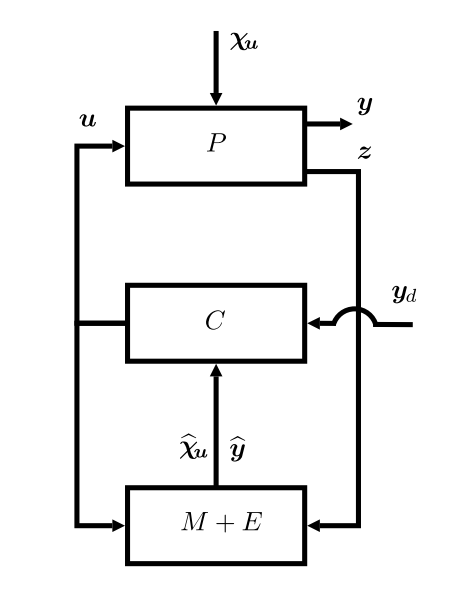
\includegraphics[scale=0.4]{images/General-control-scheme.png}
	\caption{General control scheme of constraint-based approach (source:~\cite{de2007constraint})}
	\label{fig:control}
\end{figure}

In the above figure, $P$ is \textit{plant}, that represent overall system (robot and its environment). The inputs to the system are desired control parameters such as joint positions, torques or velocities collectively represented by signal $u$ and $X_u$ representing geometric uncertainties. $y$ is the system output variables and $z$ are sensor measurements. As seen in figure (\ref{fig:control}), the input signal $u$ is distributed between C and (M + E) blocks. Here, C represents \textit{Control} block. There is another input to Control block, i.e., $y_d$, that represents desired values. The constraints imposed on system output $y$ is converted to $y_d$. Other inputs to the controller include $\widehat{ \mathcal{X}_u}$ and $\widehat y$ representing uncertainty and output estimates respectively. These estimates are produced from \textit{model update} and \textit{estimation} block (M + E)~\cite{de2007constraint}.

Initially, the approach failed to consider the unknown dynamic parameters (friction and stiffness)~\cite{de2007constraint} and inequality constraints while computing robot motions. This deficit was further overlooked and authors extended the approach to compute the resultant motions as optimization problem~\cite{decre2013extending}~\cite{decre2009extending}. 

So far, the iTaSC framework has been implemented in various robotic systems~\cite{han2017interaction},~\cite{vanthienen2011itasc},~\cite{somani2016task}. There is an open-source software\footnote{iTaSC Open-source software available at \url{https://gitlab.mech.kuleuven.be/rob-itasc}} introduced under Orocos project called iTaSC-Skill~\cite{itasc-software} that combines different iTaSC specifications. The software is also integrated in ROS. The software uses Bayesian Filtering Library (BFL) and \hyperref[kdl]{KDL} libraries to retrieve sensor data and representing virtual kinematic structure of robot. The implementation is currently controlled at velocity-level and considers only equality constraints~\cite{itasc-software}.

\section{Dynamic Modeling in Mobile Robots}

An autonomous mobile robot navigate from its current location to destination by avoiding obstacles along its way. An important consideration is the safety of robot and its environment. The researchers have introduced several methods to implement safe navigation~\cite{borenstein1990real},~\cite{adouane2011mobile}. There are few methods that consider the dynamic model to control mobile robot motions~\cite{fox1997dynamic},~\cite{asensio2002kinematic},~\cite{campion1996structural},~\cite{ge2002dynamic},~\cite{borenstein1989real}. 

The literature~\cite{fox1997dynamic} proposes \textit{dynamic window approach} that implements an effective collision avoidance technique in mobile robots with synchronous drives. The method is derived from motion dynamics. In a populated and unknown environment, a mobile robot often must react immediately to unforeseen obstacles. In such situations, the robot must dynamically re-plan so as to reach its destination.
